\documentclass[11pt,a4paper]{article}
\usepackage[a4paper,hmargin=1in,vmargin=1in]{geometry}
\usepackage{pgfplots}
\pgfplotsset{compat=1.17}

\usepackage[czech]{babel}
\usepackage[utf8]{inputenc}
\usepackage[T1]{fontenc}

\usepackage{stddoc}
\usepackage{siunitx}

\renewcommand\Re{\operatorname{Re}}
\renewcommand\Im{\operatorname{Im}}
\newcommand{\fourier}[3]{\mathcal F_{#1} \left[ #2 \right]\left( #3 \right)}
\newcommand{\ifourier}[3]{\mathcal F^{-1}_{#1} \left[ #2 \right]\left( #3 \right)}

\begin{document}

    \pagenumbering{arabic}

% Hlavička
    \begin{center}
        \section*{Materiálová disperze elektromagnetických vln}
        \vspace{-4mm}
        \begin{minipage}{0.4\textwidth}
            \begin{flushleft}
                \textsc{\today}
            \end{flushleft}
        \end{minipage}
        ~
        \begin{minipage}{0.4\textwidth}
            \begin{flushright}
                \textsc{Martin Šimák}
            \end{flushright}
        \end{minipage}
        \noindent\rule{14.5cm}{0.6pt}
    \end{center}

    \section{Materiálová disperze}

        Tentokrát se budeme zabývat chováním elektromagnetických vln v disperzních prostředích. Hlavní změnou je, že již nemůžeme předpokládat homogenní či izotropní prostředí. Nám známé materiálové vztahy tedy utrpí malou změnu:
        \begin{align}
            \vec D(\vec r,t) &= \[\epsilon \ast \vec E(\vec r)\](t),
        &
            \hat{\vec D}(\vec r,\omega) &= \hat\epsilon(\omega) \hat{\vec E}(\vec r,\omega),
        \\
            \vec B(\vec r,t) &= \[\mu \ast \vec H(\vec r)\](t),
        &
            \hat{\vec B}(\vec r,\omega) &= \hat\mu(\omega) \hat{\vec H}(\vec r,\omega),
        \\
            \vec J(\vec r,t) &= \[\sigma \ast \vec E(\vec r)\](t),
        &
            \hat{\vec J}(\vec r,\omega) &= \hat\sigma(\omega) \hat{\vec E}(\vec r,\omega),
        \end{align}
        tj. klasické násobení funkcí musíme v tomto případě nahradit konvolucí. Materiálové funkce se tedy chovají něco jako Greenovy funkce či \uv{impluzové odezvy}. Pro všechny tyto funkce musí samozřejmě platit kauzalita a stabilita, tj. vlastnosti
        \begin{align}
            f(t) &= 0 \text{ pro } t<0,
        &
            f(t) &= 0 \text{ pro } t \to \infty.
        \end{align}
        Jednou jejich další důležitou vlastností je reálnost, což implikuje symetrii Fourierova obrazu:
        \begin{align}
            \hat f(\omega) = \int_\R f(t) e^{-i\omega t} \: \d t &= \[ \int_\R f(t) e^{i\omega t} \: \d t \]^* = \hat f^*(-\omega),
        \\
            \hat f(\omega) &= \hat f^*(-\omega).
        \end{align}

    \subsection{Lorentzův disperzní model}
        Model vznikl jako historická představa materiálu jakožto soustavy hmotných kuliček v pohybu harmonického oscilátoru. Celý popis taktéž vychází z Newtonových pohybových rovnic pro harmonický oscilátor s tlumícím faktorem $\Gamma$ a rezonanční frekvencí $\omega_0$.
        \begin{align}
            \npder{2}{\vec P}{t}(t) + \Gamma \pder{\vec P}{t}(t) + \omega_0^2 \vec P(t) &= \epsilon_0 \omega_p^2 \vec E(t),
        \\
            -\omega^2 \hat{\vec P}(\omega) + i\omega \Gamma \hat{\vec P}(\omega) + \omega_0^2 \hat{\vec P}(\omega) &= \epsilon_0 \omega_p^2 \hat{\vec E}(\omega),
        \\
            \hat{\vec P}(\omega) &= \epsilon_0 \underbrace{\frac{\omega_p^2}{\omega_0^2-\omega^2+i\omega\Gamma}}_{\hat\chi_e(\omega)} \hat{\vec E}(\omega),
        \\
            \hat\epsilon(\omega) &= \epsilon_0\[1+\hat\chi_e(\omega)\],
        \\
            \hat\epsilon(\omega) &= \epsilon_0 \(1+\frac{\omega_p^2}{\omega_0^2-\omega^2+i\omega\Gamma}\),
        \\
            \hat\epsilon(\omega) &= \epsilon_0 \(1+\sum_i \frac{\omega_{p,i}^2}{\omega_{0,i}^2-\omega^2+i\omega\Gamma_i}\).
        \end{align}
        Poslední úprava je přechod k jakémusi interpolačnímu modelu, kdy zavádíme pro přesnost více parametrických tripletů $\omega_p, \omega_0, \Gamma$. Do dnešní doby je vhodným modelem pro popis velké spousty přírodních materiálů.

    \subsection{Drudeův disperzní model}
        
        Jedná se o speciální případ Lorentzova modelu s nulovou rezonanční frekvenční a s plazmovou frekvencí $\omega_p^2 = \sigma_0\Gamma/\epsilon_0$ v řádech THz.
        \begin{align}
            \hat\epsilon(\omega) &= \epsilon_0\(1-\frac{\omega_p^2}{\omega(\omega-i\Gamma)}\),
        &
            \hat\sigma(\omega) &= \frac{\sigma_0}{1+i\dfrac{\omega}{\Gamma}}.
        \end{align}
        Drudeův model se hodí pro popis kovů, kde koeficient tlumení $\Gamma$ nabývá významu \uv{srážkové frekvence}. Představme si proto jakési bezkolizní prostředí, kde $\Gamma \to 0$. Tam bude platit
        \begin{align}
            \frac{\Gamma}{\omega} &\ll 1 \quad\implies\quad \hat\epsilon(\omega) \approx \epsilon_0 \(1-\frac{\omega_p^2}{\omega^2}\).
        \end{align}
        Takové bezkolizní prostředí může být například vysokoenergetické plazma.
        \begin{figure}[!htb]
            \centering
            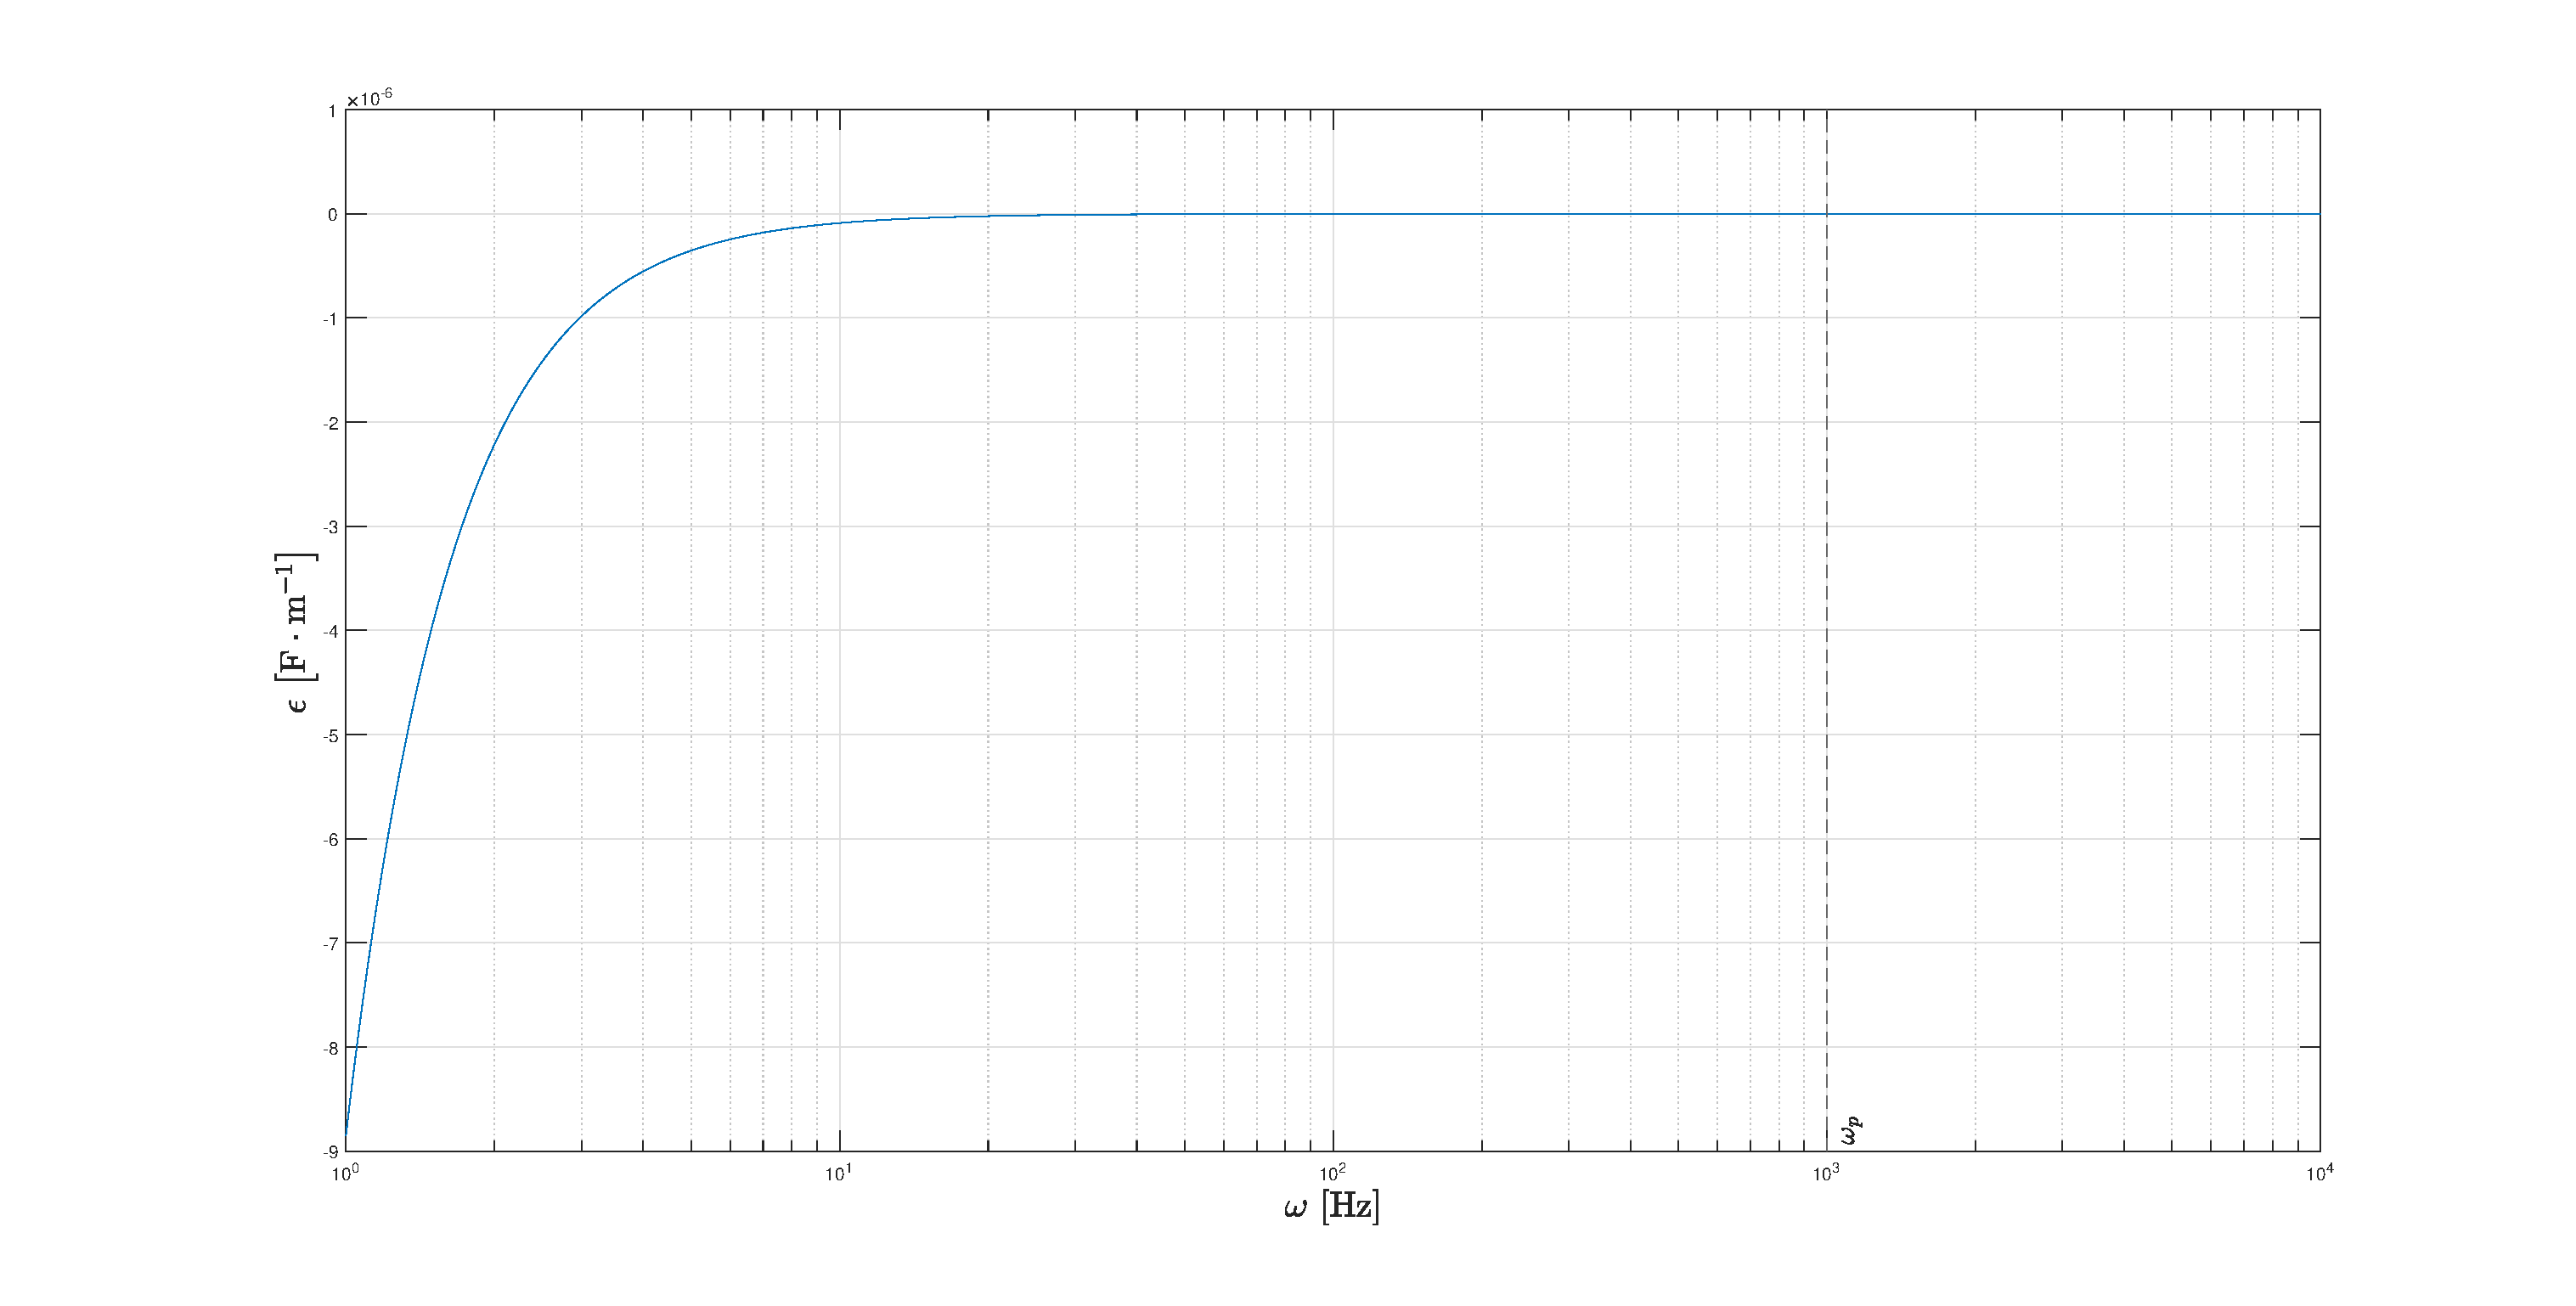
\includegraphics[width=\textwidth]{figs/drude-plasma.eps}
            \label{fig:drude-plasma}
            \caption{Graf elektrické permitivity bezkolizního ($\Gamma = 0$) materiálu v Drudeově modelu s nerealisticky nízkou plazmovou frekvencí $\omega_p = 10^3$.}
        \end{figure}

        Jak můžeme vidět, plazmová frekvence $\omega_p$ slouží jako jakási hranice, za níž je materiál pro průchod elektromagnetické vlny naprosto transparentní. To potom v praxi samozřejmě implikuje fakt, že například nemůžeme navrhovat kovové antény na vysokofrekvenční (např. RTG nebo UVC) záření. Pro nízké frekvence je permitivita záporná, což opět není překvapením, neboť v popisu elektromagnetických vln figuruje exponenciála
        \begin{align*}
            e^{ikz} = e^{i \frac{\omega}{c_0}\sqrt{\epsilon_r}z} \Big|_{\omega < \omega_p} = e^{-\frac{\omega}{c_0} \sqrt{\left|\epsilon_r\right|}z},
        \end{align*}
        tj. elektromagnetické vlny se v kovech tlumí. To z praxe očekáváme.

        V Drudeově modelu je ekvivalentní zadání elektrické permitivity $\epsilon$ nebo vodivosti $\sigma$. Pojďme se podívat například na to, jak získat vodivost ze zadané permitivity. Nejprve si vezměme některou z Maxwellových rovnic, např. Ampérův zákon s Maxwellovou korekcí:
        \begin{align*}
            \rot{\hat{\vec H}} &= \hat{\vec J} + i\omega \hat{\vec D} = \sigma \hat{\vec E} + i\omega \epsilon \hat{\vec E} = i\omega \epsilon_0 \underbrace{\(\epsilon_r + \frac{\hat\sigma}{i\omega\epsilon_0}\)}_{\tilde \epsilon_r(\omega)} \hat{\vec E}.
        \end{align*}
        Nová označená veličina $\tilde \epsilon_r$ musí odpovídat relativní permitivitě, kterou známe z Drudeova modelu, tj. musí platit, že staré $\epsilon_r = 1$ a dále
        \begin{align*}
            \frac{\hat\sigma(\omega)}{i\omega\epsilon_0} &= -\frac{\omega_p^2}{\omega(\omega-i\Gamma)}.
        \end{align*}
        Tento vztah můžeme dále upravit a zavést konstantu $\sigma_0$ jako
        \begin{align}
            \hat\sigma(\omega) &= \frac{\sigma_0}{1+i\dfrac{\omega}{\Gamma}}, \quad \sigma_0 = \hat\sigma(0) = \frac{\epsilon_0\omega_p^2}{\Gamma}.
        \end{align}

    \subsection{Debeyeův disperzní model}
        
        Tento disperzní model je relaxačním modelem $A/(1+i\omega\tau)$ s relaxační dobou $\tau$. Hodí se zejména pro popis vody a živých tkání. Jeho přesnost je však hlavně na nižších frekvencích~(řádově do desítek GHz), neboť pro vyšší frekvence se již začnou výrazně projevovat Lorentzovské odezvy. Častým příkladem Debeyeova modelu permitivity je třeba
        \begin{align}
            \hat\epsilon(\omega) &= \epsilon_0\(1+\frac{\epsilon_{r,s}-1}{1+i\omega\tau}\),
        \end{align}
        kde $\epsilon_{r,s} = \hat\epsilon_r(0)$ je \uv{stejnosměrná} relativní permitivita.

    \subsection{Appletonův disperzní model}
        
        \subsubsection{Odvození}
        
        Appletonův model je korekcí Drudeova modelu pro popis plazmatu ve vnějších slupkách atmosféry (ionosféra). Komplikací je zde samozřejmě relativně silné magnetické pole Země způsobující anizotropii. Představme si tedy zmagnetizované plazma v ionosféře: vyskytují se zde kationty a anionty, přičemž kationty jsou vcelku nepohyblivé, takže jejich interakce zanedbáme. Zajímejme se tedy rovnou o Lorentzovu sílu působící na rychlé anionty. Pro tu můžeme napsat Newtonovy pohybové rovnice bez vzájemných interakcí pro $N$ částic:
        \begin{align*}
            m_i \nder{2}{\vec r_i}{t} &= -e \vec E - e \der{\vec r_i}{t} \times \vec B_0,
        \\
            m_i \nder{2}{e\vec r_i}{t} &= -e \( e\vec E + \der{e\vec r_i}{t} \times \vec B_0\).
        \end{align*}
        Rovnici jsme si upravili tak, že se sugestivně objevuje elektrický dipól aniontů $\vec p_i = e\vec r_i$. Dále si již uvědomme, že pro všechna $i \in \{1,2,\dots,N\}$ je $m_i=m_e$. Dále se pokusme rovnici vyprůměrovat přes zkoumaný objem $V$, tj. pišme
        \begin{align*}
            m_e \underbrace{\frac 1V \sum_i \nder{2}{\vec p_i}{t}}_{\p_{tt}\vec P} = -e \bigg( e \underbrace{\frac 1V \sum_i \vec E}_{\vec E} + \underbrace{\frac 1V \sum_i \der{\vec p_i}{t}}_{\p_t \vec P} \times \vec B_0 \bigg).
        \end{align*}
        V závorce jsou uvedená zjednodušení: vektor elektrické polarizace $\vec P$ je přímo definován průměrovacím integrálem/sumou a jelikož jsou naše sumy konečné, můžeme na základě linearity derivace prohodit operace pro zjednodušení. Dále vektor elektrické intenzity $\vec E$ je přes objem zhruba konstantní, a tak ho můžeme jednoduše vyprůměrovat opět na sebe. Rovnice tedy po zavedení konstant nabývá tvaru
        \begin{align}
            \nder{2}{\vec P}{t} + \omega_c \der{\vec P}{t} \times \vec e_{B} &= \epsilon_0 \omega_p^2 \vec E,
        \end{align}
        kde $\omega_c = B_0 e/m_e$ a $\omega_p^2 = e^2/(m_e \epsilon_0)$ jsou cyklotronová a plazmová frekvence respektive. Pojďme se tedy pokusit takovou rovnici analyzovat pod Fourierovou transformací: nejprve zaveďmě souřadnicovou soustavu tak, aby $\vec e_B = \vec e_z$. Dále pišme
        \begin{align}
            -\omega^2 \hat{\vec P} + i\omega\omega_0 \hat{\vec P} \times \vec e_z &= \epsilon_0 \omega_p^2 \hat{\vec E}.
        \end{align}
        Na první pohled je vidět, že díky vektorovému součinu $\hat{\vec P} \times \vec e_z = \hat P_y \vec e_x - \hat P_x \vec e_y$ ztrácíme možnost oddělit jednotlivé složky vektorů. Dostáváme tedy vektorovou rovnici
        \begin{align*}
            -\omega^2 \begin{pmatrix}
                \hat P_x \\ \hat P_y \\ \hat P_z
            \end{pmatrix} + i\omega \omega_c \begin{pmatrix}
                \hat P_y \\ -\hat P_x \\ 0
            \end{pmatrix} &= \epsilon_0 \omega_p^2 \begin{pmatrix}
                \hat E_x \\ \hat E_y \\ \hat E_z
            \end{pmatrix},
        \\
            \begin{pmatrix}
                -\omega^2 & i \omega \omega_c  & 0
            \\
                -i\omega \omega_c & -\omega^2 & 0
            \\
                0 & 0 & -\omega^2
            \end{pmatrix} \hat{\vec P} &= \epsilon_0 \omega_p^2 \hat{\vec E},
        \\
            \hat{\vec P} &= \epsilon_0 \underbrace{\omega_p^2 \begin{pmatrix}
                -\omega^2 & i \omega \omega_c  & 0
            \\
                -i\omega \omega_c & -\omega^2 & 0
            \\
                0 & 0 & -\omega^2
            \end{pmatrix}^{-1}}_{\hat\chi_e} \hat{\vec E}
        \end{align*}
        Výpočtem inverzní matice získáváme Appletonův model permitivity
        \begin{align}
            \hat\epsilon(\omega) &= \epsilon_0 \begin{pmatrix}
                1- \frac{\omega_p^2}{\omega^2 - \omega_c^2} & -\frac{i \omega_c \omega_p^2}{\omega(\omega^2-\omega_c^2)} & 0
            \\
                \frac{i \omega_c \omega_p^2}{\omega(\omega^2-\omega_c^2)} & 1- \frac{\omega_p^2}{\omega^2 - \omega_c^2} & 0
            \\
                0 & 0 & 1- \frac{\omega_p^2}{\omega^2}
            \end{pmatrix}
        \end{align}
        jakožto antisymetrický tenzor, který díky antisymetrii vykazuje nereciproké chování. Můžeme povšimnout triviálního příkladu, kdy vyšleme vlnu kolno na atmosféru. Vektory $\hat{\vec B}_0$ a $\hat{\vec E}$ jsou potom rovnoběžné a vektorový součin $\hat{\vec P} \times \hat{\vec B}_0$ je nulový. V tomto případě dostáváme opět permitivitu jako jednoduchou skalární funkci z Drudeova modelu.

        \subsubsection{Lze v Appletonově modelu rozkládat do rovinných vln?}
        V této podsekci se budeme zabývat otázkou, jak je na tom nás elementární rozklad do rovinných vln v případě, že se nacházíme v materiálu popsaném Appletonovým disperzním modelem. Nejprve předpokládejme, že ano: Napišme si tedy Maxwellovy transformace pod plnou Fourierovou transformací.
        \begin{align}
            i \vec k \cdot \(\epsilon(\omega) \hat{\vec E}(\vec k, \omega)\) &= 0,
        \\
            i\vec k \times \hat{\vec E}(\vec k,\omega) &= -i\omega \mu_0 \hat{\vec H}(\vec k,\omega),
        \\
            i \vec k \cdot \hat{\vec H}(\vec k,\omega) &= 0,
        \\
            i\vec k \times \hat{\vec H}(\vec k,\omega) &= i \omega\epsilon(\omega) \hat{\vec E}(\vec k,\omega).
        \end{align}
        Klasickou kombinací druhé a čtvrté rovnice získáme vztah
        \begin{align*}
            \vec k \times \(-\frac{1}{\omega \mu_0} \vec k \times \hat{\vec E}\) &= \omega \epsilon(\omega) \hat{\vec E},
        \\
            \vec k \times \(\vec k \times \hat{\vec E}\) &= \omega^2 \mu_0 \epsilon_0 \epsilon_r(\omega) \hat{\vec E},
        \\
            -\(\vec k \cdot \hat{\vec E}\)\vec k + \norm{k}^2 \hat{\vec{E}} &= k_0^2 \epsilon_r(\omega) \hat{\vec E}.
        \end{align*}
        Zásadní změnou zde však je, že nemusí nutně platit $\vec k \cdot \hat{\vec E} = 0$. Speciální případ: $\hat{\vec E} = (\hat E_x,\hat E_y,0)^{\mathrm T}$, $\vec k = k_z \vec e_z$. To be continued.
        

\end{document}